% Introduction and/or Motivation - 15 pts
For decades, Gantt charts have been used by High Performance Computing (HPC) professionals to profile and analyze the execution of highly-parallel programs running on multiple cores. When profiling, developers are looking for "bottlenecks" in code, or places where parallelism is not as effective as it could be. A common cause of bottlenecks is the useless work being done transferring data or waiting on the execution of processes: "overhead." Gantt charts, showing the parallel execution of many processes over time, are very good for rendering communications between processes with lines showing how long communication took, when it began and where it ends. This notation gives developers a clear topology of how their program is communicating and guides them to opportunities for optimization.

Unfortunately, this reliance on Gantt charts and lines to denote communication poses a unique problem. Where once nearly half of supercomputers in the top 500 of the world had 16 or fewer cores \cite{top500}, a naive approach to developing these visualizations worked well. In Figure \ref{fig:simple_gantt}, we see an example of such a visualization. As supercomputers have grown to thousands and tens-of-thousands of cores however, this approach of visualizing execution traces is no longer effective.

As we can see in Figure \ref{fig:bad_gantt} significant meaning is lost from this chart when it is scaled up into the 100s of cores. Most importantly, it is impossible to see the individual lines connecting calls between processes. They are lost entirely in a sea of visual noise. Even though this software provides functionality to zoom in and explore subsections in greater detail, it is of little value if one cannot determine the key areas to examine. The visualization no longer provides an effective high level view which can be used to quickly identify key message passing patterns and potential bottlenecks.


\begin{figure}[h]
    \centering
    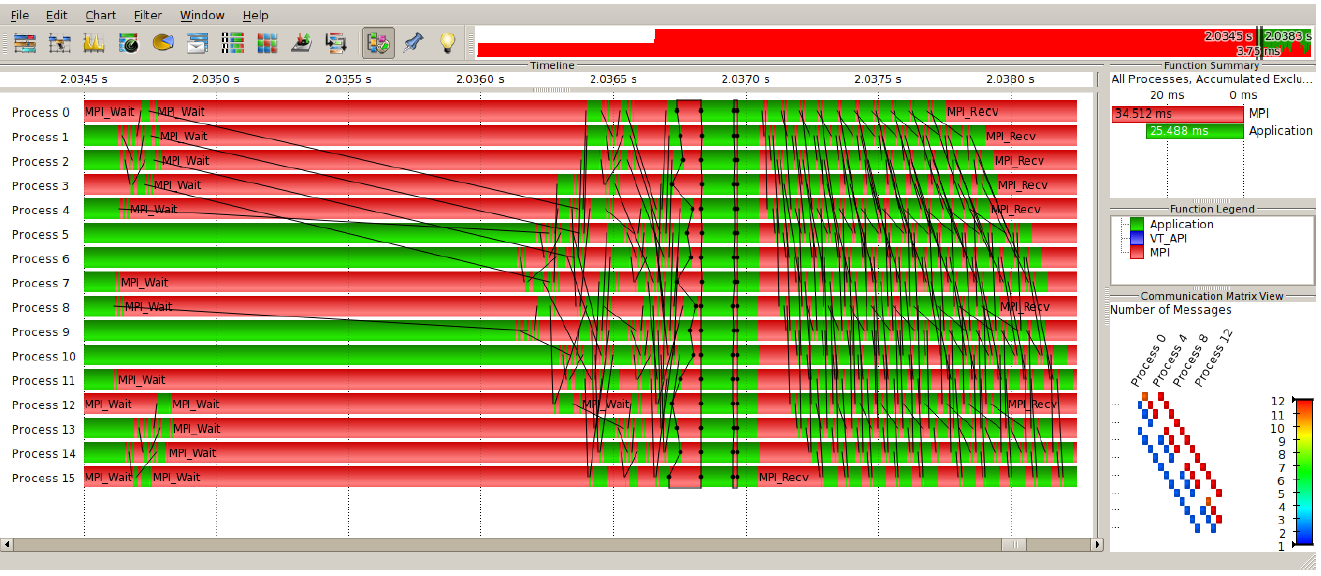
\includegraphics[width=.4\textwidth]{figs/basic_gantt.png}
    \caption{A Gantt chart produced by Vampir from \cite{isaacs2014state}. Functions invoked with the MPI library are shown in red and other executions are indicated with green. The y axes organizes bars by process and the x axis shows execution states of each process over time. Black lines connecting bars show communication between processes via passes messages.}
    \label{fig:simple_gantt}
\end{figure}

What this example shows is that Gantt charts do not scale to meet contemporary needs in HPC. Critical information provided by patterns of message passing lines cannot be rendered at this resolution. This failure provokes the question which drives the subject of this paper: How can we render all the necessary and sufficient communications data required to find potential problems in massively parallel HPC programs within the physical limitations posed by dense charts? What marks are redundant? What marks are necessary? If we can answer these questions, this work will provide a firm foundation upon which to design a more effective visualization for HPC profiling. This in turn, will positively impact the productivity of parallel programmers seeking to optimize critical software.

\begin{figure}[h]
    \centering
    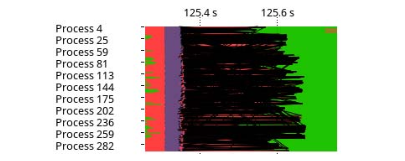
\includegraphics[width=.53\textwidth]{figs/bad_gantt.png}
    \caption{A Gantt chart produced by Vampir from \cite{Brendel2016}. Lines intended to show communication between processes are too numerous to be parsed meaningfully. Furthermore these lines obscure other parts of the chart.}
    \label{fig:bad_gantt}
\end{figure}

In the domain of HPC visualization, and with communication lines on Gantt charts especially, the appropriate balance of necessary and sufficient information is not clearly defined. To address this gap, we propose an empirical study examining how effectively people recognize patterns of lines which simulate message-call patterns in real Gantt charts. This experiment will be implemented as a within-subjects study, evaluating how error rates of pattern recognition are affected by how much of an overall pattern is provided. Does a partial representation of a pattern provide enough meaningful information? Is a full representation too much? What is the threshold between the two? Does the pattern itself impact what marks are redundant or necessary?

This study can provide valuable granular information about what characteristics users identify or lock-on to when processing visual patterns. It can inform possible designs by showing when users can no longer recognize meaningful patterns or by showing how little a user requires for identification and recognition. 

To summarize, the aims of this research are:
\begin{enumerate}
    \item Develop and execute a visualization user study 
    \item Evaluate the results of said user study and draw meaningful conclusions about:
    \begin{enumerate}
        \item People's ability to recognize patterns of the variety commonly found in the lines denoting message passing in line charts
        \item Glean what information is redundant in communication visualizations without suffering significant loss of meaning.
    \end{enumerate}
\end{enumerate}

